\documentclass[11pt,addpoints]{exam}
\usepackage{amsfonts,amssymb,amsmath, amsthm}
\usepackage{graphicx}
\usepackage{systeme}
\usepackage{pgf,tikz,pgfplots}
\pgfplotsset{compat=1.15}
\usepgfplotslibrary{fillbetween}
\usepackage{mathrsfs}
\usetikzlibrary{arrows}
\usetikzlibrary{calc}
\usepackage{enumitem}
\setlist[itemize]{leftmargin=5em} % Adjust the indent size as desired
\usepackage{listings}
\newcommand{\codefont}{\fontfamily{pcr}\selectfont}
\lstdefinestyle{mystyle}{
  basicstyle=\codefont\footnotesize,   % Set the font and size
  numbers=left,                 % Line numbers on the left
  numberstyle=\tiny,            % Style of line numbers
  stepnumber=1,                 % Line number increment
  numbersep=5pt,                % Distance between line numbers and code
  backgroundcolor=\color{gray!10}, % Background color
  frame=single,                 % Frame around the code
  rulecolor=\color{gray},       % Color of frame
  breaklines=true,              % Break long lines
  breakatwhitespace=true,       % Break lines at whitespace
  showstringspaces=false,       % Don't show spaces in strings
  upquote=true,                 % Use straight quotes
  commentstyle=\color{green},   % Style of comments
  keywordstyle=\color{blue},    % Style of keywords
  stringstyle=\color{orange}    % Style of strings
}
\lstnewenvironment{code}{\lstset{language=R}}{}
% \qformat{}
\renewcommand{\thepartno}{\arabic{partno}}
\@addtoreset{partno}{question}
\pagestyle{headandfoot}

\firstpageheader{Midterm Exam: Take-home (\numpoints\ points)\\ March 2024}{}{Name: \underline{Eli Orians\hspace{2.5in}}}
%\firstpageheadrule

\runningheader{Final Exam}{}{Page \thepage\ of \numpages}
\runningheadrule

\firstpagefooter{}{}{}
\runningfooter{}{}{}


\begin{document}

\begin{center}
\fbox{\fbox{\parbox{6in}{
Handwritten answers are unacceptable; you must type your answers after each question. For this purpose, use the TEX file and submit the PDF file.  To receive full credit, you must show all of your work. For programming questions, you must submit your code as well. Your code must generate your answer without any error messages. This exam has one extra point ($\max=25$).
}}}
\end{center}


%------ # 1 ------%
\begin{questions}
\question[5]{Consider a linear transformation given by the matrix
\[
A = \begin{bmatrix}
-1 & 0 & 0 & 0 \\
1 & 1 & 0 & 0 \\
2 & 5 & 2 & 1 \\
-1 & 1 & 0 & 3 \\
\end{bmatrix}.
\]
Find a basis for \(\mathbb{R}^4\) with respect to which the matrix representation for the linear transformation above is diagonal.}\\

To find the basis for \(\mathbb{R}^4\) such that $A$ is diagonal, we will start by finding the eigenvalues of $A$. So we will solve the equation: $\text{{det}}(A - \lambda I) = 0$

\[
\text{{det}}\left(\begin{bmatrix}
-1 & 0 & 0 & 0 \\
1 & 1 & 0 & 0 \\
2 & 5 & 2 & 1 \\
-1 & 1 & 0 & 3 \\
\end{bmatrix} - \lambda \begin{bmatrix}
1 & 0 & 0 & 0 \\
0 & 1 & 0 & 0 \\
0 & 0 & 1 & 0 \\
0 & 0 & 0 & 1 \\
\end{bmatrix}\right) = 0
\]

\[
\text{{det}}\left(\begin{bmatrix}
-1 - \lambda & 0 & 0 & 0 \\
1 & 1 - \lambda & 0 & 0 \\
2 & 5 & 2 - \lambda & 1 \\
-1 & 1 & 0 & 3 - \lambda \\
\end{bmatrix}\right) = 0
\]

Next, begin by swapping rows 1 and 2 to change the sign of the determinate.

\[
= -\text{det}\begin{bmatrix}
1 & 1-\lambda & 0 & 0 \\
-1-\lambda & 0 & 0 & 0 \\
2 & 5 & 2 - \lambda & 1 \\
-1 & 1 & 0 & 3 - \lambda \\
\end{bmatrix}
\]
Add $(\lambda + 1) * $row 1 to row 2.
\[
= -\text{det}\begin{bmatrix}
1 & 1-\lambda & 0 & 0 \\
0 & 1-\lambda^2 & 0 & 0 \\
2 & 5 & 2 - \lambda & 1 \\
-1 & 1 & 0 & 3 - \lambda \\
\end{bmatrix}
\]
Subtract 2 * row 1 from row 3.
\[
= -\text{det}\begin{bmatrix}
1 & 1-\lambda & 0 & 0 \\
0 & 1-\lambda^2 & 0 & 0 \\
0 & 3+2\lambda & 2 - \lambda & 1 \\
-1 & 1 & 0 & 3 - \lambda \\
\end{bmatrix}
\]
Add row 1 to row 4.
\[
= -\text{det}\begin{bmatrix}
1 & 1-\lambda & 0 & 0 \\
0 & 1-\lambda^2 & 0 & 0 \\
0 & 3+2\lambda & 2 - \lambda & 1 \\
0 & 2-\lambda & 0 & 3 - \lambda \\
\end{bmatrix}
\]

Add $\frac{3 + 2\lambda}{1 - \lambda^2}$ * row 2 to row 3.
\[
= -\text{det}\begin{bmatrix}
1 & 1-\lambda & 0 & 0 \\
0 & 1-\lambda^2 & 0 & 0 \\
0 & 0 & 2 - \lambda & 1 \\
0 & 2-\lambda & 0 & 3 - \lambda \\
\end{bmatrix}
\]

Add $-\frac{2 -\lambda}{1 - \lambda^2}$ * row 2 to row 4.
\[
= -\text{det}\begin{bmatrix}
1 & 1-\lambda & 0 & 0 \\
0 & 1-\lambda^2 & 0 & 0 \\
0 & 0 & 2 - \lambda & 1 \\
0 & 0 & 0 & 3 - \lambda \\
\end{bmatrix}
\]

The determinant of an upper triangular matrix is the product of its diagonal elements. Therefore,
\[ = -(1-\lambda^2)(2-\lambda)(3-\lambda)\]
\[ = \lambda^4 - 5\lambda^3 + 5\lambda^2 + 5\lambda - 6  \]
\[\lambda = 3, 2, 1, -1 \]

Next, we find the eigenvectors by solving $(A - \lambda I)v = 0$ for each eigenvalue. 

For $\lambda  = 3$:
\[
\left(\begin{bmatrix}
-4 & 0 & 0 & 0 \\
1 & -2 & 0 & 0 \\
2 & 5 & -1 & 1 \\
-1 & 1 & 0 & 0 \\
\end{bmatrix}\right)v = 0
\]

Multiply both sides by an invertible matrix to get a reduced row echelon form.
\[
\left(
\begin{bmatrix}
0 & -1 & 0 & -2 \\
0 & -1 & 0 & -1 \\
0 & -7 & -1 & -9 \\
1 & -4 & 0 & -8 \\
\end{bmatrix}
\begin{bmatrix}
-4 & 0 & 0 & 0 \\
1 & -2 & 0 & 0 \\
2 & 5 & -1 & 1 \\
-1 & 1 & 0 & 0 \\
\end{bmatrix}\right)v = 
\begin{bmatrix}
0 & -1 & 0 & -2 \\
0 & -1 & 0 & -1 \\
0 & -7 & -1 & -9 \\
1 & -4 & 0 & -8 \\
\end{bmatrix}0
\]

\[
\left(\begin{bmatrix}
1 & 0 & 0 & 0 \\
0 & 1 & 0 & 0 \\
0 & 0 & 1 & -1 \\
0 & 0 & 0 & 0 \\
\end{bmatrix}\right)v = 0
\]

\begin{align*}
x1 = 0\\
x2 = 0\\
x3 - x4 = 0
\end{align*}

\begin{align*}
x1 = 0\\
x2 = 0\\
x3 = x4
\end{align*}

\[ So,
v = \begin{bmatrix}
0 \\
0 \\
1 \\
1
\end{bmatrix}
\]

Repeating this process for the other eigenvalues...

For $\lamda$ = 2

\[
v = \begin{bmatrix}
0 \\ 
0 \\ 
1 \\ 
0 \\
\end{bmatrix}
\]

For $\lamda$ = 1:

\[
x = \begin{bmatrix}
0 \\ 
-2 \\ 
9 \\ 
1 \\
\end{bmatrix}
\]

For $\lamda$ = -1:

\[
x = \begin{bmatrix}
24 \\ 
-12 \\ 
1\\
9 \\
\end{bmatrix}
\]

Using the eigenvectors we will create the matrix P.

\[
P = \begin{bmatrix}
24 & 0 & 0 & 0 \\
-12 & -2 & 0 & 0 \\
1 & 9 & 1 & 1 \\
9 & 1 & 0 & 1 \\
\end{bmatrix}
\]

Finally, we will test if this matrix is linearly independent to see if it is a basis of A. Performing row reduction we get:

\[
P = \begin{bmatrix}
1 & 0 & 0 & 0 \\
0 & 1 & 0 & 0 \\
0 & 0 & 1 & 0 \\
0 & 0 & 0 & 1 \\
\end{bmatrix}
\]

Since all columns of P are linearly independent, the eigenvectors form a basis for matrix A.

%------ # 2 ------%

\question[2]{Find the nullspace of
\[
A = \begin{bmatrix}
4 & -2 & 0 \\
2 & 1 & -1 \\
2 & -3 & 1 \\
\end{bmatrix}
\]
}

To begin, we will reduce the matrix to row echelon form. The first step in this process is to subtract 1/2 * row 1 from row 2

\[
A = \begin{bmatrix}
4 & -2 & 0 \\
0 & 2 & -1 \\
2 & -3 & 1 \\
\end{bmatrix}
\]

Add row 2 to row 3.

\[
A = \begin{bmatrix}
4 & -2 & 0 \\
0 & 2 & -1 \\
0 & 0 & 0 \\
\end{bmatrix}
\]

Divide row 2 by 2.

\[
A = \begin{bmatrix}
4 & -2 & 0 \\
0 & 1 & -1/2 \\
0 & 0 & 0 \\
\end{bmatrix}
\]

Add 2 * row 2 to row 1.

\[
A = \begin{bmatrix}
4 & 0 & -1 \\
0 & 1 & -1/2 \\
0 & 0 & 0 \\
\end{bmatrix}
\]

Lastly, divide row 1 by 4 to get the following matrix in reduced row echelon form. Note the free variable $x_3$ that will be used later.

\[
A = \begin{bmatrix}
1 & 0 & -1/4 \\
0 & 1 & -1/2 \\
0 & 0 & 0 \\
\end{bmatrix}
\]

Next, we will solve for $A v = 0$ using the reduced matrix.

\[
A = \begin{bmatrix}
1 & 0 & -1/4 \\
0 & 1 & -1/2 \\
0 & 0 & 0 \\
\end{bmatrix}
\begin{bmatrix}
x_1\\
x_2\\
x_3 \\
\end{bmatrix} =
\begin{bmatrix}
x_1-x_3/4 \\
x_2-x_3/2\\
0 \\
\end{bmatrix}.
\]

Convert this to a system of equations.

\begin{align*}
x_1 = x_3/4\\
x_2 = x_3/2\\
0 = 0
\end{align*}

Rewrite v using the free variable $x_3$, reassigned as $x$.

\[\begin{bmatrix}
x/4 \\
x/2\\
x \\
\end{bmatrix}\]

Since $x$ is taken from \mathbb{R}, we can replace it with $4x$ resulting in:

\[\begin{bmatrix}
x \\
2x\\
4x \\
\end{bmatrix}\]

Therefore, the null space for the matrix A is

\[ (x, 2x, 4x) : x \in \mathbb{R} \]\\

% ------ # 3 ------%

\question{
Consider the vector norm \(\| \cdot \|_1\) on \(\mathbb{R}^n\) given by \(\|x\|_1 = \sum_{i=1}^{n} |x_i|\), where \(x = [x_1, \ldots, x_n]^T\). Define the norm \(\| \cdot \|_1\) on \(\mathbb{R}^m\) similarly. 

\begin{parts}
\part[3] Show that the matrix norm induced by these vector norms is given by

\[\|A\|_1 = \max_{k} \sum_{i=1}^{m} |a_{ik}|\]

where \(a_{ij}\) is the \((i, j)\)th element of \(A \in \mathbb{R}^{m \times n}\).
%\textbf{Hint:} First, for each $x$ such that \(\|x\|_1 = 1\) show that \[
%\|Ax\|_1 \leq \max_{k} \sum_{i=1}^{m} |a_{ik}|,
%\]
%Then, find (define) an $x*$ such that \(\|x^*\|_1 = 1\) and $\|Ax^*\|_1 = \max_{k} \sum_{i=1}^{m} |a_{ik}|.$
\\
To show that the matrix norm induced by the $\| \cdot \|_1$ vector norm is given by

\[\|A\|_1 = \max_{k} \sum_{i=1}^{m} |a_{ik}|,\]

we need to establish two things:

\begin{enumerate}
    \item For any $x$ such that $\|x\|_1 = 1$, we need to show that $\|Ax\|_1 \leq \max_{k} \sum_{i=1}^{m} |a_{ik}|$.
    \item There exists an $x$ such that $\|x\|_1 = 1$ for which $\|Ax\|_1 = \max_{k} \sum_{i=1}^{m} |a_{ik}|$.
\end{enumerate}


\begin{enumerate}
\item Starting with the first premise, let $x$ be any vector such that $||x||_1 = 1$. Then we have,
\[||Ax||_1 = \sum_{i=1}^{m} |(Ax)_i|\]
Now consider $||Ax||_1$
\[||Ax||_1 = \sum_{i=1}^{n} |\sum_{j=1}^{m} a_{ij}x_j|\]
Using triangle inequality, we can write:
\[||Ax||_1 <= \sum_{i=1}^{n} \sum_{j=1}^{m} |a_{ij}x_j|\]
Since the absolute value function is non-negative, we can interchange the order of summation
\[||Ax||_1 <= \sum_{j=1}^{m} \sum_{i=1}^{n} |a_{ij}x_j|\]
Now, notice that for each $j$, we have $\sum_i=1^{n}|a_{ij}x_j|<= \max{k} \sum_i=1^{m}|a_{ik}|$. Therefore,
\[||Ax||_1 <= \max_{k} \sum_{i=1}^{m}|a_{ik}|\]

Therefore, $||Ax||_1 <= \max_{k} \sum_{i=1}^m|a_{ik}|$ holds for each x such that $||x||_1 = 1$\\

\item To satisfy the second premise, let $x^*$ be the column of A that corresponds to the maximum value of $\sum_{i=1}^{m}|a_{ik}|$. More formally, let $k^*$ be the index that achieves the maximum value $k^* = \max{k}\sum_{i=1}^m|a_{ik}|$. So, $x^*$ will be the following matrix where 1 is in the $k^*$th position:

\[\begin{bmatrix}
    0 \\ ... \\ 0 \\ 1 \\ 0 \\ ... \\ 0
\end{bmatrix}\]

Now calculate $||Ax^*||_1$
\[||Ax^*||_1 = \sum_{i=1}^{n} |\sum_{j=1}^{m} a_{ij}x^*_j|\]
Since $x^*$ has only one non-zero element, we can simplify the above expression to:
\[||Ax^*||_1 = \sum_{i=1}^{n} |a_i k^*|\]
Remember that $k* = \max{k}\sum_{i=1}^m|a_{ik}|$ so,
\[||Ax^*||_1 = \sum_{i=1}^{n} |a_i k^*| = \max{k}\sum_{i=1}^m|a_{ik}|\]
Therefore, the matrix norm induced by the vector norm $||\cdot||_1$ is given by $||Ax^*||_1 = \max{k}\sum_{i=1}^m|a_{ik}|$\\
\end{enumerate}

\part[3] Find the induced matrix norm of the identity matrix $I_n$, the orthogonal matrix $Q_n$, and a positive definite symmetric matrix $A_n$ based on $\|A\|_1$ norm defined in the previous part.

To find the induced matrix norm of the identity matrix $I_n$, we will use the formula from the previous section.
\[||A||_1 = \max{k}\sum_{i=1}^{m} |a_i k|\]
For the identity matrix, all the elements on the main diagonal are 1 and all other elements are 0. Therefore, in each column, there is only one non-zero element with a value of 1.  So,  $\sum_{i=1}^{m}$ will be 1. Since this is the maximum value we can obtain for any column, we have:
\[||I_n||_1 = \max{k}\sum_{i=1}^{m} |a_i k| = 1\]

For the orthogonal matrix $Q_n$, the columns are orthonormal, meaning that each column has a norm of 1 and the dot product between any two columns is 0. Therefore, for each column $k$ of $Q_n$, the sum will be 1. Again, this is the maximum value we can obtain for any column, so we have: 
\[||Q_n||_1 = \max{k}\sum_{i=1}^{m} |a_i k| = 1\]

For a positive definite symmetric matrix $A_n$, the maximum value of $\sum_{i=1}^{m} |a_i k|$ will be equal to the sum of the absolute values of the largest eigenvalue of $A_n$. Therefore, we have:
\[||A_n||_1 = \max{k}\sum_{i=1}^{m} |a_i k| = \text{largest eigenvalue}\]
\end{parts}
}

%------ # 4 ------%

\question{Consider the problem
\[
\begin{aligned}
& \text{minimize}
& & f(x) \\
& \text{subject to}
& & x \in \Omega,
\end{aligned}
\]
where \( f: \mathbb{R}^2 \rightarrow \mathbb{R} \) is given by \( f(x) = -3x_1 \) with \( x = [x_1, x_2]^T \), and \( \Omega = \{x = [x_1, x_2]^T : x_1 + x_2^2 \leq 2\} \). Answer each of the following questions, showing complete justification.

\begin{parts}
    \part[1] Does the point \( x^* = [2, 0]^T \) satisfy the first-order necessary condition? Why?\\

    The first order necessary condition for $x*$ requires that there exist a scalar $\lambda >= 0$ such that 
    \[\nabla f(x^*) + \lambda \nabla g(x^*) = 0\]
    
    We begin by finding the gradient of f(x).

    \[\nabla f(x) = 
    \begin{bmatrix} 
    -3 \\ 0 
    \end{bmatrix}\]

    \[\nabla f(x^*) = 
    \begin{bmatrix} 
    -3 \\ 0 
    \end{bmatrix}\]

    Next, we find the gradient of the constraint function, rewritten as: $g(x) = x_1 + x_2^2 -2$

    \[\nabla g(x) = 
    \begin{bmatrix} 
    1 \\ 2x_2 
    \end{bmatrix}\]

    \[\nabla g(x^*) = 
    \begin{bmatrix} 
    1 \\ 0
    \end{bmatrix}\]

    Then, we will use these values in the original formula and solve for $\lambda$.

    \[\begin{bmatrix} -3 \\ 0 \end{bmatrix} + \lambda \begin{bmatrix} 1 \\ 0 \end{bmatrix} = \begin{bmatrix} 0 \\ 0 \end{bmatrix}\]

    \[ \begin{bmatrix} -3 + \lambda \\ 0 \end{bmatrix} + \lambda \begin{bmatrix} 1 \\ 0 \end{bmatrix} = \begin{bmatrix} 0 \\ 0 \end{bmatrix}\]

    \[\lambda = 3\]

    Since $\lambda >= 0$, the scalar multiplier condition is satisfied. Therefore the point $x^*$ does satisfy the first-order necessary condition. \\

    \part[1] Does the point \( x^* = [2, 0]^T \) satisfy the second-order necessary condition? Why?\\

    Since the function $f(c) = -3x_1$ is linear, its Hessian matrix is a zero matrix.  The second-order necessary condition states that for a local minimum at $x^*$, the Hessian matrix of $f$ at $x^*$ must be positive semi-definite on the tangent space of the constraints at $x^*$.

    \[\nabla^2 f(x) = 
    \begin{bmatrix} 
    0 & 0 \\ 0 & 0
    \end{bmatrix}\]

    The zero matrix is positive semi-definite. Therefore, the point $x*$ satisfies the second-order necessary condition for any constraint set including \( \Omega = \{x = [x_1, x_2]^T : x_1 + x_2^2 \leq 2\} \).\\

    \part[1] Is the point \( x^* = [2, 0]^T \) a local minimizer? Why?\\

    Because the point $x*$ satisfies both the first-order and second-order necessary conditions under the constraint $x_1 + x_2^2 -2 = 0$, $x*$ is a local minimizer.
    
\end{parts}
}
\clearpage
\question{[\textbf{Python Programming}]
Let \(f(x) = x^2 + 4 \cos x\), \(x \in \mathbb{R}\). We wish to find the minimizer \(x^*\) of \(f\) over the interval \([1,2]\). (\textit{Calculator users: Note that in} \(\cos x\), \textit{the argument} \(x\) \textit{is in radians. Truncate your results with four decimal points.})

%------ # 5 ------%

\begin{parts}
\part[1] Plot \(f(x)\) versus \(x\) over the interval \([1,2]\).
    \begin{figure}[h]
        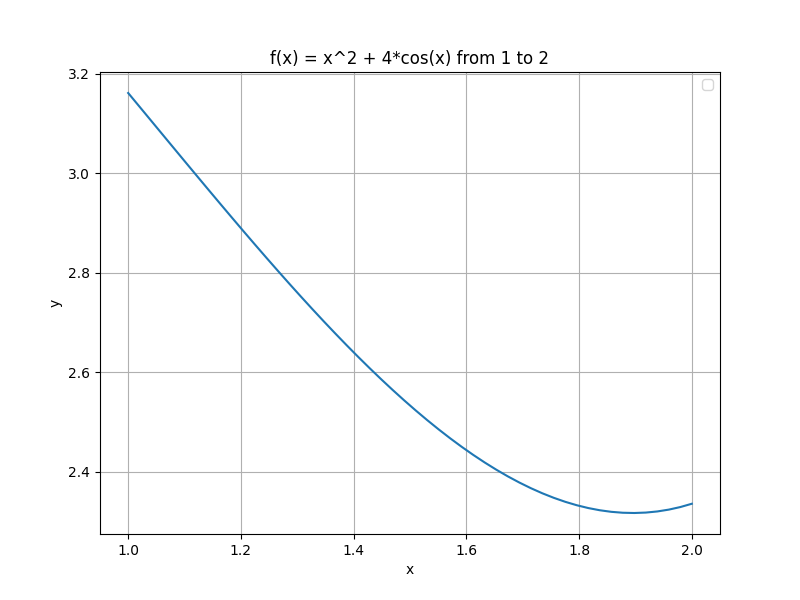
\includegraphics[width=1\linewidth]{plot.png}
    \end{figure}

\part[3] Use the golden section method to locate \(x^*\) to within an uncertainty of 0.2. Display all intermediate steps using a table:
\begin{center}
\begin{tabular}{c c c c c c}
\hline
Iteration \(k\) & \(a_k\) & \(b_k\) & \(f(a_k)\) & \(f(b_k)\) & New uncertainty interval \\
\hline
1 & 1.00 & 2.0 & 2.66 & 2.429 & \([1.00, 2.00]\) \\
2 & 1.38 & 2.0 & 2.42 & 2.343 & \([1.38, 2.00]\) \\
3 & 1.61 & 2.0 & 2.34 & 2.319 & \([1.61, 2.00]\) \\
4 & 1.76 & 2.0 & 2.31 & 2.317 & \([1.76, 2.00]\) \\
5 & 1.85 & 2.0 & 2.31 & 2.317 & \([1.85, 2.00]\) \\
\hline
\end{tabular}
\end{center}


\part[3] Repeat part b using the Fibonacci method, with \(\epsilon = 0.05\). Display all intermediate steps using a table:
\begin{center}
\begin{tabular}{c c c c c c c}
\hline
Iteration \(k\) & \(\rho_k\) & \(a_k\) & \(b_k\) & \(f(a_k)\) & \(f(b_k)\) & New uncertainty interval \\
\hline
1 & 0.38 & 1.00 & 2.0 & 2.66 & 2.428 & \([1.00, 2.00]\) \\
2 & 0.38 & 1.38 & 2.0 & 2.42 & 2.344 & \([1.38, 2.00]\) \\
3 & 0.37 & 1.61 & 2.0 & 2.34 & 2.319 & \([1.61, 2.00]\) \\
4 & 0.40 & 1.76 & 2.0 & 2.31 & 2.316 & \([1.76, 2.00]\) \\
5 & 0.33 & 1.85 & 2.0 & 2.31 & 2.322 & \([1.85, 2.00]\) \\
6 & 0.50 & 1.85 & 1.95 &2.31 & 2.316 & \([1.85, 1.95]\) \\
7 & 0.50 & 1.90 & 1.95 &2.31 & 2.316 & \([1.90, 1.95]\) \\
\hline
\end{tabular}
\end{center}


\part[3] Apply Newton's method, using the same number of iterations as in part b, with \(x^{(0)} = 1\).
\end{parts}
}

\end{questions}
\end{document}